\documentclass{article}
\usepackage{titling}
\usepackage[T1]{fontenc}
\usepackage[polish]{babel}
\usepackage[utf8]{inputenc}
% Margins in document
\usepackage[left=1.5cm, right=1.5cm, top=3cm]{geometry}

% Avoid  colons before tables' empty captions and change caption
\usepackage{caption}
\captionsetup[table]{name=Tab.}
\captionsetup[figure]{name=Rys.}

% Don't know why, it starts from 2
\addtocounter{table}{-1}

% Rename tables' suffix
\renewcommand{\tablename}{Tab.}

% Graphicx setup
\usepackage{graphicx}
\graphicspath{{grafiki/}{../grafiki/}}

% No separator between items
\usepackage{enumitem}
\setlist{nolistsep}

% Pagebreak before every \section
\let\oldsection\section
\renewcommand\section{\clearpage\oldsection}

% Vhistory setup
\usepackage[owncaptions]{vhistory}
\renewcommand{\vhhistoryname}{Historia zmian}
\renewcommand{\vhversionname}{Wersja}
\renewcommand{\vhdatename}{Data}
\renewcommand{\vhauthorname}{Autor(zy)}
\renewcommand{\vhchangename}{Zmiany}

% Bigger padding in tabulars
\usepackage{array}
\setlength\extrarowheight{3pt}

% Itemize in tabulars (avoid big margins with minipage)
\newcommand{\tabbeditemize}[1]{
	\begin{minipage}[t]{0.4\textwidth}
		\begin{itemize}[topsep=0mm,partopsep=0mm,leftmargin=4mm]
			#1
		\end{itemize}
\end{minipage}}


% DOCUMENT
\title{
	Wizualizacja drzewa stanów algorytmu UCT \\
	\large Plan projektu}

\author{Patryk Fijałkowski \\ Grzegorz Kacprowicz}
\begin{document}
	\begin{titlingpage}
		\maketitle
		\vspace{3cm}
		\begin{abstract}
			Poniższy dokument zawiera ogólny zarys projektu-aplikacji. Składa się on z opisu architektury systemu i poszczególnych komponentów wraz z pełnioną funkcją. Opisane są tu interfejsy skłądających się na ten projekt modułów, użyte biblioteki i komunikacja między nimi. Znajdują się tu też diagramy UML, które opisują klasy w projekcie i ich zachowanie względem siebie. Dokument zawiera również przykładowy interfejs graficzny dla użytkownika. Co więcej, opisane są użyte technologie i wymagania sprzętowe.
		\end{abstract}
	\end{titlingpage}

	\begin{versionhistory}
		\vhEntry{1.0}{3.11.2019}{PF|GK}{stworzenie pierwszej wersji dokumentu}
	\end{versionhistory}
	
	\tableofcontents
	
	\section{Architektura aplikacji}
	Aplikacja będzie podzielona na 5 oddzielnych modułów: algorytm, serializacja, wizualizacja, gra 1, gra 2... Ten odpowiedzialny za to, tamten za to... Takie rozwiązanie jest dobre bo...
	
	
	\section{Moduły aplikacji}
	Szczegółowy opis każdego z modułów w subsection...
	
	
	\section{Główne komponenty aplikacji}
	Najważniejsze komponenty:
	\begin{itemize}
		\item MonteCarloTreeSearch, BaseGameMove, BaseGameState
		\item BaseSerializator, BinarySerializator, CsvSerializator
		\item MonteCarloNode, MonteCarloNodeDetails, MonteCarloVisualisationDetails
	\end{itemize}
	
	\section{Interfejs użytkownika}
	Menu:
	\begin{figure}[h!]
		\centering
		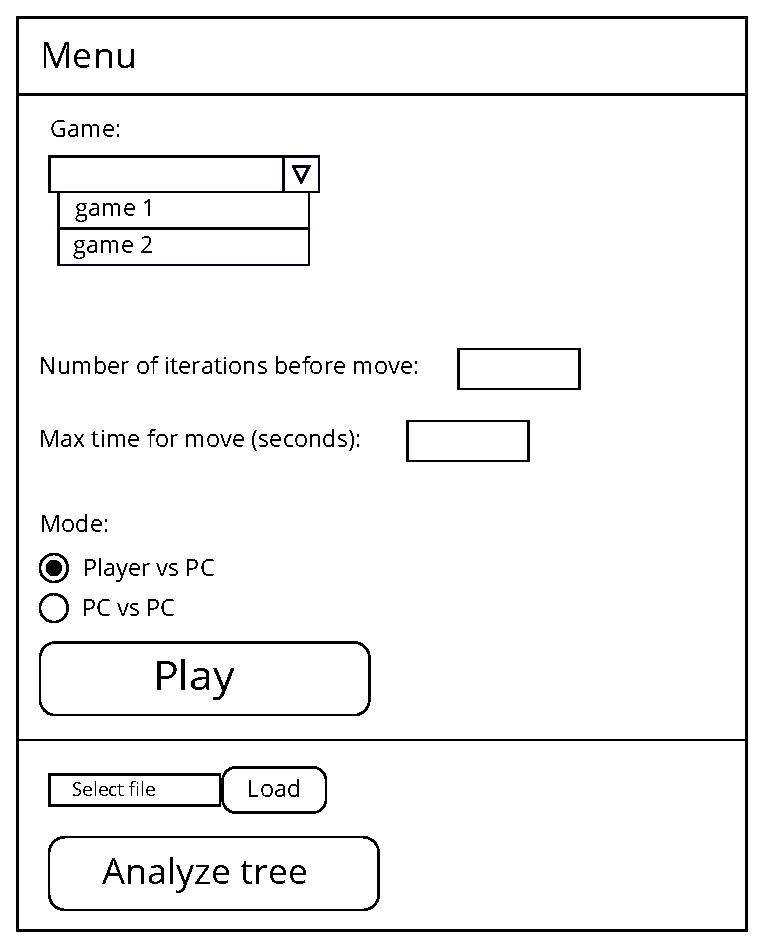
\includegraphics[scale=0.8, trim={18.8cm 0 0 0},clip]{menu-eps}
	\end{figure}\\
	Analiza drzewa:
	\begin{figure}[h!]
		\centering
		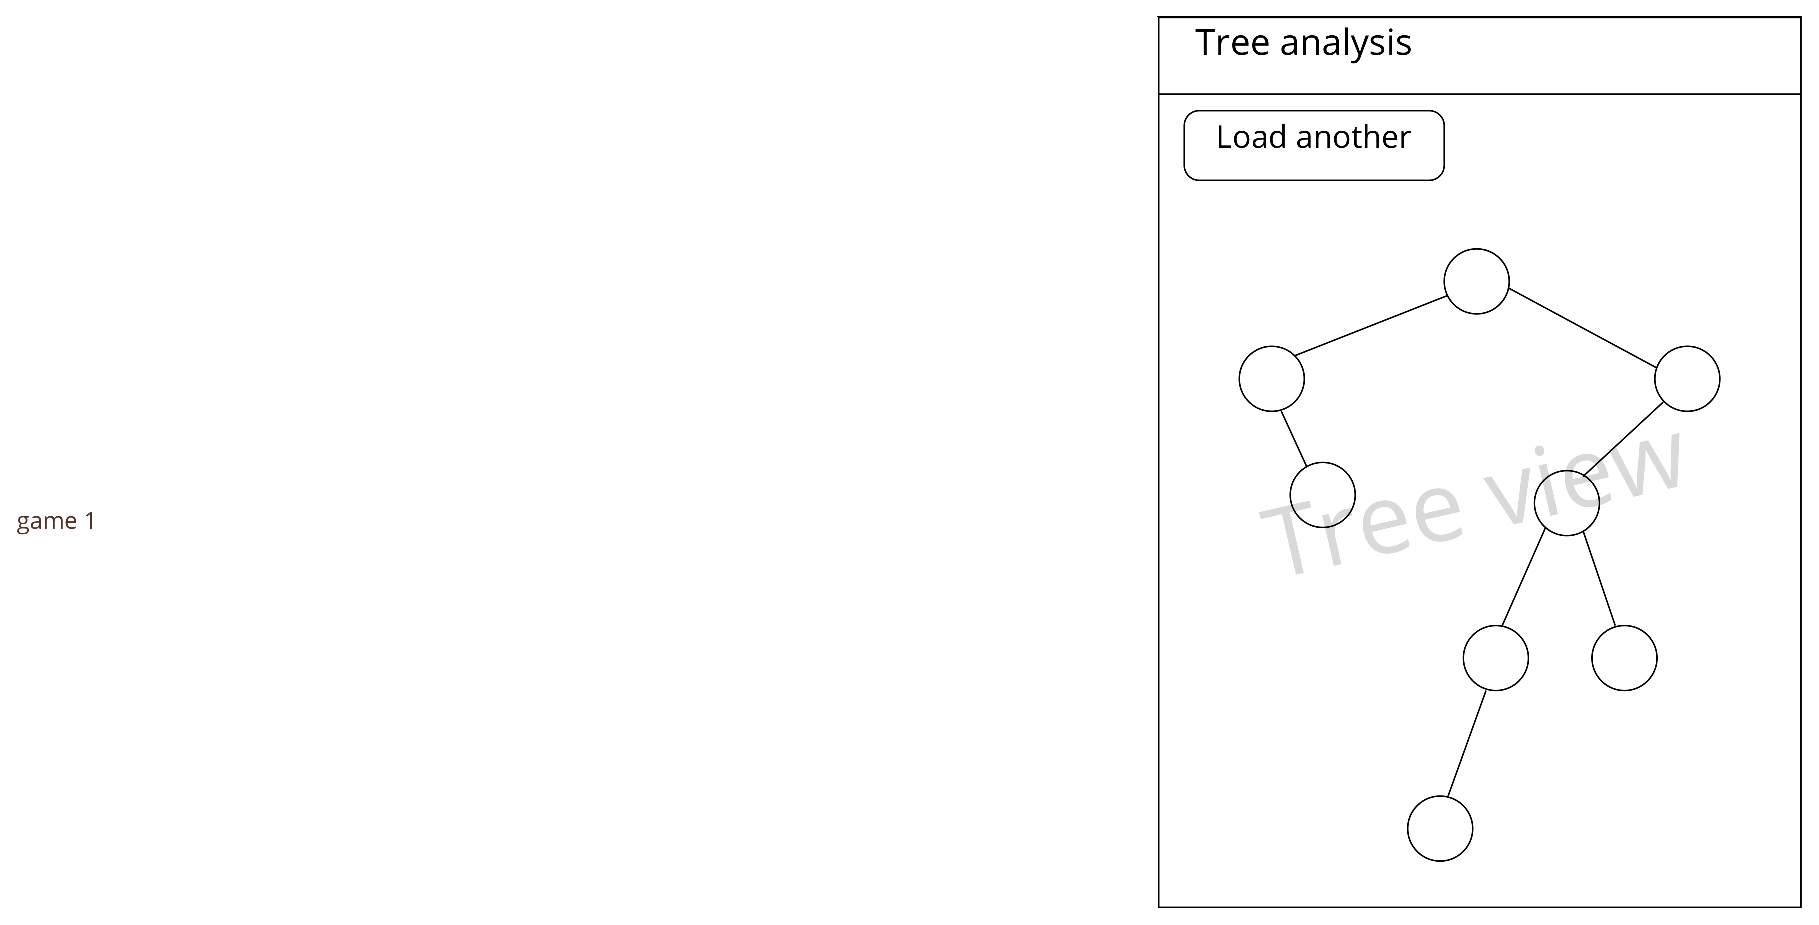
\includegraphics[scale=0.8, trim={18cm 0 0 0},clip]{analyze-eps}
	\end{figure}
	\pagebreak\\
	Rozgrywka:
	\begin{figure}[h!]
		\centering
		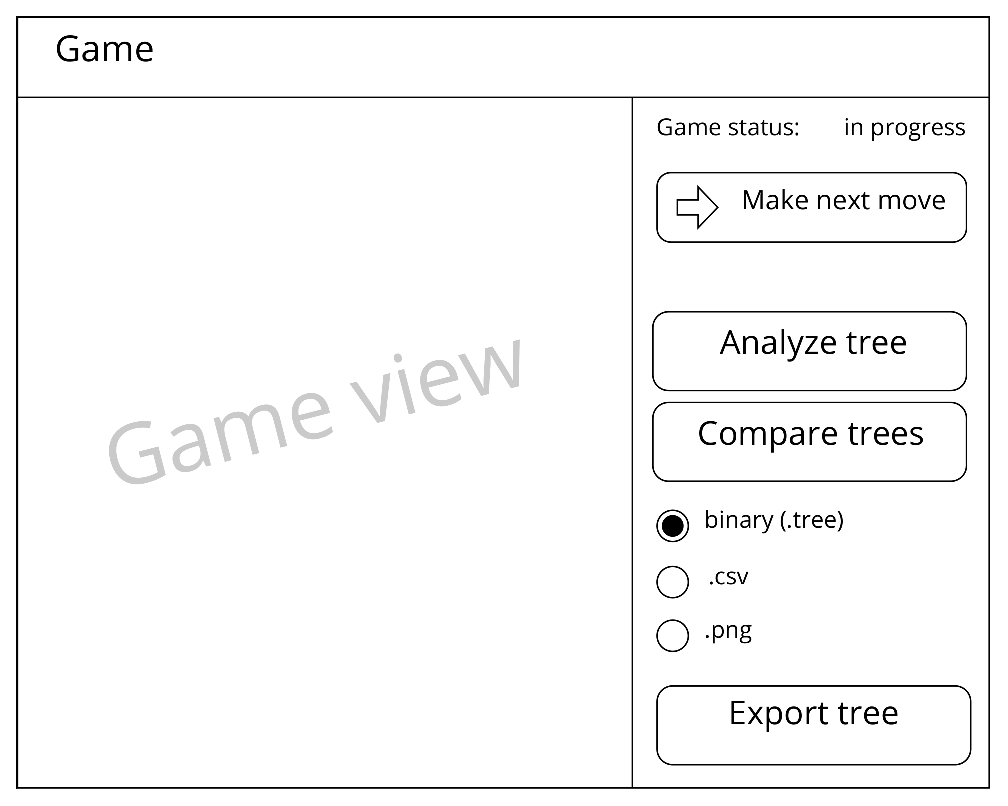
\includegraphics[scale=0.8]{game-eps}
	\end{figure}
	
	\section{Wybrane technologie}
	Wybraną przez nas technologią do napisania aplikacji tj.: gier, algorytmu i wizualizacji jest język programowania \textbf{Python} w stabilnej wersji 3.7. Do implementacji gier będziemy posługiwać się biblioteką \textbf{PyGame} (w wersji stabilnej). Wizualizacja będzie wykorzystywać w znacznym stopniu bibliotekę \textbf{VisPy} (OpenGL), w której najbardziej przydatną dla nas funkcją będzie możliwość pisania kodu w języku \textbf{C++} i stosunkowo łatwa integracja z głównym językiem projektu - Pythonem. Wykorzystana przez nas wersja tej biblioteki również będzie wersją stabilną.\\
	
	\noindent Python został przez nas wybrany ze względu na swoją wszechstronność. Posiada on bardzo szeroki zakres bibliotek, co pozwoli nam napisać zdecydowaną większość kodu w jednym języku i przyspieszyć wymianę informacji między komponentami (np. kodem gier a kodem algorytmu MCTS).\\
	
	\noindent VisPy jest nową technologią, która jest wciąż rozwijana, jednak została przez nas wybrana głównie ze względu na:
	\begin{itemize}
		\item współpracę z GPU, co będzie niezbędne podczas wizualizacji setek tysięcy wierzchołków grafu,
		\item obszerną dokumentację,
		\item brak lepszej alternatywy.\\
	\end{itemize}
	Wybór na PyGame padł ze względu na:
	\begin{itemize}
		\item łatwość pisania kodu i przemyślane API,
		\item popularność i dobrą dokumentację.\\
	\end{itemize}
	Program ma w założeniu działać na komputerze osobistym, który posiada kartę graficzną.\\
	Aplikacja działa na systemach operacyjnych Windows i Linux.
	
\end{document}